\section{The \sys{} System}
\label{sec:system}

\sys{} is a monocular, zero-shot FIG D-scoring pipeline. Given a raw
competition video, it detects and tracks the athlete, segments the run into
individual tricks, sends each trick clip to a vision--language model with
a FIG-grounded prompt, snaps the model's free-form trick name to the official
FIG table via a fuzzy matcher, and assembles a D-score card for the run.
Figure~\ref{fig:architecture} shows the overall flow. The system is
deliberately modular: the VLM is replaceable and every stage has a testable
text-level interface.

\begin{figure*}[t]
  \centering
  % Figure 2: PkVision system architecture (full-width TikZ).
% Included directly in sections/03_system.tex via \input.

\resizebox{\textwidth}{!}{%
\begin{tikzpicture}[
    node distance=5mm and 5mm,
    font=\small,
    >={Stealth[round]},
    every node/.style={align=center},
    stage/.style={draw, rounded corners=2pt, thick, minimum height=10mm, minimum width=22mm, fill=cvprblue!10},
    data/.style ={draw, rounded corners=2pt, thick, minimum height=9mm, minimum width=20mm, fill=gray!8, dashed},
    arrow/.style={-Stealth, thick, cvprblue!80!black},
]

% --- Row: pipeline stages left-to-right
\node[data]  (video)    {Competition\\video};
\node[stage, right=of video]     (track)   {YOLO-pose\\tracking};
\node[stage, right=of track]     (seg)     {Inversion\\segmentation};
\node[stage, right=of seg]       (clip)    {Per-trick\\clip};
\node[stage, right=of clip]      (vlm)     {VLM\\(Claude / Gemini /\\open-weights)};
\node[stage, right=of vlm]       (match)   {Fuzzy FIG\\matcher};
\node[stage, right=of match]     (score)   {D-score\\assembler};
\node[data,  right=of score]     (out)     {FIG\\scorecard};

% --- Arrows
\draw[arrow] (video) -- (track);
\draw[arrow] (track) -- (seg);
\draw[arrow] (seg)   -- (clip);
\draw[arrow] (clip)  -- (vlm);
\draw[arrow] (vlm)   -- node[above,font=\scriptsize]{free-form name} (match);
\draw[arrow] (match) -- node[above,font=\scriptsize]{FIG name + D-score} (score);
\draw[arrow] (score) -- (out);

% --- Annotations below a couple of stages
\node[font=\scriptsize, below=1mm of track, text=gray!60!black]
    {\texttt{core/video.py}};
\node[font=\scriptsize, below=1mm of seg, text=gray!60!black]
    {\texttt{core/segmentation.py}};
\node[font=\scriptsize, below=1mm of vlm, text=gray!60!black]
    {\texttt{core/vlm/*}};
\node[font=\scriptsize, below=1mm of match, text=gray!60!black]
    {5-level cascade};

\end{tikzpicture}%
}

  \caption{\textbf{\sys{} architecture.} A raw monocular run passes through
  YOLO-pose athlete tracking, inversion-based segmentation, and per-clip VLM
  judging. A five-level fuzzy matcher snaps each free-form VLM name to the
  official FIG Table of Tricks, and the D-score assembler produces a
  scorecard. Arrows show the flow of a single trick through the pipeline;
  every box has a text-level interface and can be swapped in isolation.}
  \label{fig:architecture}
\end{figure*}

\subsection{Athlete Tracking and Inversion Segmentation}
\label{sec:system:segmentation}

Parkour competition footage usually contains a single athlete performing a
continuous line of tricks, interrupted by running, setup, and crowd
reactions. We use YOLO-pose~\cite{jocher2023yolo} on every frame (module
\texttt{core/video.py}) and keep the detection that is both largest in area
and closest to the previously tracked bounding box centre, producing a
single stable track for the athlete. Per-frame signals we retain are the
nose $y$, hip midpoint $y$, and torso inclination angle derived from the
shoulder--hip vector.

Each FIG acrobatic trick has the same signature: during the aerial phase
the athlete becomes at least partially \emph{inverted}~--- the head passes
below the hips in image coordinates. We exploit this to segment the run
without ever computing a 3D pose. Concretely, for each frame $t$ we compute
the inversion signal
\begin{equation}
i_t = \max(0, y^{\text{head}}_t - y^{\text{hip}}_t),
\end{equation}
normalise it by the 90th percentile of its positive values, and smooth with
a $0.1\,\text{s}$ box kernel. A second smoothed signal $a_t$ measures
frame-to-frame angular velocity of the torso, wrapped into $[0,\pi]$.
The combined score $s_t = 0.7\, \tilde\imath_t + 0.3\, \tilde a_t$ is
thresholded to mark active frames; contiguous active regions become candidate
segments, padded by $0.3\,\text{s}$ on each side, merged if closer than
$0.4\,\text{s}$, and filtered to the $[0.3, 4.0]\,\text{s}$ duration window.
A segment is kept only if it contains at least one inverted frame or a
strong rotational burst (\texttt{core/segmentation.py}, lines 27--145).

The design deliberately avoids any appearance-based classifier. The
inversion cue is language- and clothing-invariant, does not depend on
apparatus type, and fails gracefully under heavy camera motion
(Sec.~\ref{sec:experiments}). Figure~\ref{fig:segmentation} visualises the
three signals and the resulting segments on \texttt{IMG\_5985.mov}.

\begin{figure}[t]
  \centering
  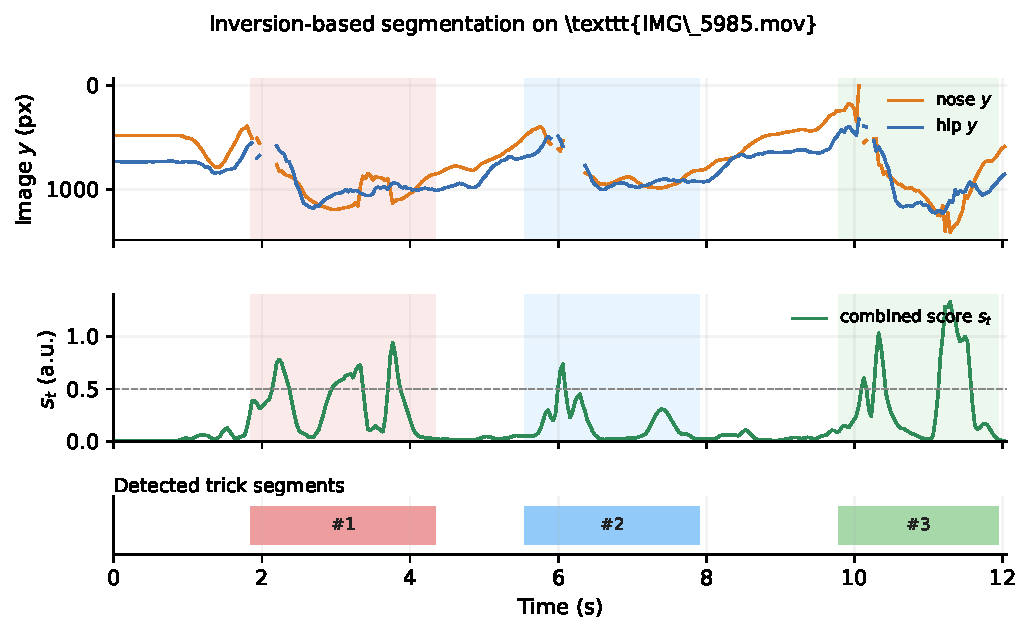
\includegraphics[width=\linewidth]{figures/fig03_segmentation.pdf}
  \caption{\textbf{Inversion-based segmentation on a real run.}
  Top: nose $y$ (orange) and hip $y$ (blue). Middle: smoothed combined score
  $s_t$. Bottom: detected segments (shaded). The three acrobatic tricks in
  \texttt{IMG\_5985.mov} (Gainer Full, Krok, Double Cork) are cleanly
  isolated from run-ups and crowd transitions.}
  \label{fig:segmentation}
\end{figure}

\subsection{Vision--Language Model Prompting}
\label{sec:system:vlm}

Each candidate segment is re-encoded as a short MP4 and submitted to a
vision--language model through a common \texttt{VLMProvider} interface
(\texttt{core/vlm/base.py}). We implement three concrete providers:
Gemini~\cite{team2024gemini} accepts the clip natively as a video input,
Claude~\cite{anthropic2024claude3} and OpenAI models receive eight uniformly
sampled key frames, and OpenRouter routes the same interface to a pool of
open-weight models such as Qwen2-VL~\cite{bai2023qwen} and
Kimi-VL~\cite{moonshot2024kimi}.

The prompt is constructed once per run from
\texttt{core/vlm/prompt.py} and is identical across providers for a fair
comparison. It contains three sections (Figure~\ref{fig:prompt}): (i) a
markdown table of the 149 official FIG tricks with their physical
properties (flips, twists, direction, category, aliases), (ii) a manually
curated disambiguation guide for visually confusable tricks (e.g., backflip
vs.\ gainer vs.\ palm flip), and (iii) a strict JSON response schema asking
for trick name, category, direction, flip count, twist count, confidence
level, and free-text reasoning. The prompt never names the target clip or
its expected answer; the VLM must ground every identification in the
submitted frames or video.

\begin{figure}[t]
  \centering
  % Figure 4: Prompt structure (column-wide TikZ).

\begin{tikzpicture}[
    font=\small,
    >={Stealth[round]},
    box/.style={draw, rounded corners=2pt, thick, align=left, text width=6.6cm, inner sep=4pt},
    header/.style={font=\small\bfseries, cvprblue!80!black},
    arrow/.style={-Stealth, thick, cvprblue!80!black},
    every node/.style={align=left},
]

\node[box, fill=cvprblue!6] (role) {%
    \textbf{Role} \\
    \scriptsize\emph{``You are an expert FIG parkour judge. Identify every
    trick in this competition run.''}
};

\node[box, fill=cvprblue!10, below=4mm of role] (tab) {%
    \textbf{FIG Trick Table (149 entries)} \\[1pt]
    \scriptsize
    {\ttfamily | Name | Flips | Twists | Direction | Category |} \\
    {\ttfamily | Back Flip | 1 | 0 | back | acrobatics |} \\
    {\ttfamily | Gainer Full | 1 | 1 | back | acrobatics |} \\
    {\ttfamily | Double Cork | 2 | 2 | back | acrobatics |} \\
    {\ttfamily ... 146 rows ...}
};

\node[box, fill=cvprblue!14, below=4mm of tab] (dis) {%
    \textbf{Disambiguation Guide} \\[1pt]
    \scriptsize
    Same physics (1 flip, 0 twist, back): \\
    \quad Back Flip --- two-foot standing takeoff \\
    \quad Gainer --- one-foot running takeoff \\
    \quad Palm Flip --- hand contact on takeoff
};

\node[box, fill=cvprblue!18, below=4mm of dis] (schema) {%
    \textbf{Strict JSON Response Schema} \\[1pt]
    \scriptsize\ttfamily
    \{"tricks": [\{"trick\_name": ..., \\
    \hspace*{1em}"category": ..., "direction": ..., \\
    \hspace*{1em}"flip\_count": ..., "twist\_count": ..., \\
    \hspace*{1em}"confidence": ..., "reasoning": ...\}]\}
};

\draw[arrow] (role.south)  -- (tab.north);
\draw[arrow] (tab.south)   -- (dis.north);
\draw[arrow] (dis.south)   -- (schema.north);

\end{tikzpicture}

  \caption{\textbf{Prompt structure.} Every provider receives the same
  three-part message: the full FIG Table of Tricks, a disambiguation guide
  for visually confusable variants, and a strict JSON response schema. The
  VLM returns one JSON record per identified trick; its free-form name is
  then fuzzy-matched against the FIG table in the next stage.}
  \label{fig:prompt}
\end{figure}

Parsing is robust to markdown fences, stray prose, and truncated JSON: we
extract the first balanced \texttt{\{...\}} block and accept any that
satisfies the minimum schema. A consensus mode
(\texttt{core/vlm/consensus.py}) queries $N$ models in parallel and returns
the modal FIG name along with an agreement score; we report both
single-model and consensus numbers in Sec.~\ref{sec:experiments}.

\subsection{The Five-Level Fuzzy FIG Matcher}
\label{sec:system:matcher}

VLMs happily emit names such as ``Gainer Full 360'', ``Corkscrew'', ``back
full twist'', or ``double half cork''. These are all valid colloquial
references to tricks in the FIG table, but none are exact FIG names.
Without a matcher, VLMs would be penalised for stylistic rather than
semantic errors. The \texttt{FIGMatcher} (\texttt{core/vlm/fig\_matcher.py})
is a deterministic five-level cascade, shown in Figure~\ref{fig:matcher},
that snaps any free-form name to one of the 149 FIG entries or declines to
match:

\begin{enumerate}
  \item[\textbf{L1}] \textbf{Exact match} (case-insensitive) against the
        FIG name index.
  \item[\textbf{L2}] \textbf{Alias match} against the curated alias lists
        embedded in \texttt{fig\_tricks\_2025.json} (e.g., ``Ginger''
        $\rightarrow$ ``Palm Backflip'').
  \item[\textbf{L3}] \textbf{Normalised match}: rewrite informal tokens
        (\emph{full}$\rightarrow$360, \emph{half}$\rightarrow$180,
        \emph{double full}$\rightarrow$720, \ldots) and retry L1 in both
        directions.
  \item[\textbf{L4}] \textbf{Jaccard token overlap}: the highest-overlap
        FIG name wins if its Jaccard similarity exceeds $0.5$.
  \item[\textbf{L5}] \textbf{Physics fallback}: if the VLM reports flip and
        twist counts, pick the unique FIG entry with the same
        $(\text{flip}, \text{twist}, \text{direction})$; if several match,
        prefer the highest D-score.
\end{enumerate}

\begin{figure}[t]
  \centering
  % Figure 5: Fuzzy FIG matcher 5-level cascade with worked example.

\resizebox{\columnwidth}{!}{%
\begin{tikzpicture}[
    font=\small,
    >={Stealth[round]},
    level/.style={draw, rounded corners=2pt, thick, minimum width=1.6cm, minimum height=8mm, align=center, fill=cvprblue!10},
    hit/.style  ={draw, rounded corners=2pt, thick, minimum width=1.6cm, minimum height=8mm, align=center, fill=green!15},
    miss/.style ={draw, rounded corners=2pt, thick, minimum width=1.6cm, minimum height=8mm, align=center, fill=gray!8, dashed},
    arrow/.style={-Stealth, thick, cvprblue!80!black},
    ex/.style={font=\scriptsize\ttfamily, text=gray!60!black},
]

% Input on the left
\node[miss] (in) {VLM output\\\scriptsize\texttt{"back full twist"}};

\node[miss, right=3mm of in] (l1) {L1\\exact};
\node[miss, right=2mm of l1] (l2) {L2\\alias};
\node[hit,  right=2mm of l2] (l3) {L3\\normalised};
\node[level,right=2mm of l3] (l4) {L4\\Jaccard};
\node[level,right=2mm of l4] (l5) {L5\\physics};

\node[hit, right=3mm of l5] (out) {FIG name\\\textbf{Back Full}\\\scriptsize D$=2.0$};

% Arrows
\draw[arrow] (in)  -- (l1);
\draw[arrow] (l1)  -- (l2);
\draw[arrow] (l2)  -- (l3);
\draw[arrow] (l3)  -- (l4);
\draw[arrow] (l4)  -- (l5);
\draw[arrow] (l5)  -- (out);

% "Match found" dashed arrow
\draw[arrow, dashed, cvprblue!60!black]
    (l3.south) to[out=-90,in=-90,looseness=0.6] (out.south);

\end{tikzpicture}%
}

  \caption{\textbf{The five-level fuzzy matcher.} Free-form VLM output
  is snapped to an official FIG name via a deterministic cascade. A worked
  example (\emph{``back full twist''} $\rightarrow$ L3 normalised
  $\rightarrow$ \textbf{Back Full}) is shown. Every match records its
  level, which we report as an ablation in Table~\ref{tab:matcher_levels}.}
  \label{fig:matcher}
\end{figure}

The cascade is fully auditable: each match records which level produced it,
which lets us report (Table~\ref{tab:matcher_levels}) how much of the
benchmark accuracy is carried by the matcher versus the VLM itself. We show
in Sec.~\ref{sec:experiments} that removing the matcher drops
trick-top-1 accuracy substantially, which is why we argue the matcher is a
first-class contribution and not just glue code.

\subsection{D-Score Assembly}
\label{sec:system:dscore}

The final stage applies the FIG scoring rules to the list of matched
tricks. FIG rewards only a run's top-3 difficulty contributions in the
final D-score, so \sys{} sums the three highest matched base values and
emits a scorecard with per-trick reasoning, match level, and the total.
Repeated tricks do not count even if their form, entry, or exit differ, as
per the 2025 Code of Points~\cite{fig2025codepoints}; the assembler
deduplicates by FIG name. Failed tricks (those the VLM flags with confidence
\texttt{low}) are reported but excluded from the total, matching FIG's
$-4.00$ / $-6.00$ deduction rule. The scorecard is the system's final
output; an example is shown in Figure~\ref{fig:scorecards}.

\begin{table}[t]
  \centering
  \small
  % Auto-generated by paper/scripts/make_tables.py; do not edit.
\begin{tabular}{lrr}
\toprule
Level & Hit rate & Match confidence \\
\midrule
L1 exact         & 100.0\% & 1.00 \\
L2 alias         & 0.0\% & 1.00 \\
L3 normalised    & 0.0\% & 0.85--0.90 \\
L4 Jaccard       & 0.0\% & $\geq$0.50 \\
L5 physics       & 0.0\% & 0.50--0.70 \\
unmatched        & 0.0\% & --- \\
\midrule
\textbf{total}   & 21 calls & --- \\
\bottomrule
\end{tabular}

  \caption{\textbf{Fuzzy matcher cascade hit rate} on POOL-B.
  Most VLM outputs already match at L1 (exact) or L3 (normalised); the
  token-overlap and physics fallback levels absorb informal names that
  would otherwise be scored as wrong. See Sec.~\ref{sec:experiments}.}
  \label{tab:matcher_levels}
\end{table}
